\section{Généralité}
Dans le monde réel, la lumière est un phénomène complexe.
Une partie de la lumière vient d’une direction ou d’une position particulière, alors
qu’une autre partie est généralement dispersée sur l’ensemble de la scène. En optique,on la modélise comme étant un assemblage de 4 composantes :
\begin{itemize}
\item Lumière ambiante
\item Lumière diffuse
\item Lumière spéculaire
\item Lumière émissive
\end{itemize}

\section{Lumière ambiante}
\begin{center}
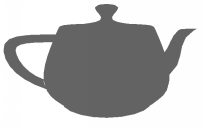
\includegraphics[width=5cm,height=5cm]{pipeline/images/objet_ambiante.png}
\end{center}
Cette composante n'a pas source précise, elle provient de tous les points de la scène.
\\\\
Elle ne permet pas à elle seule de voir les détails des objets de la scène car elle éclaire toute la scène de la même façon, sans ombre.
\\\\
\begin{center}
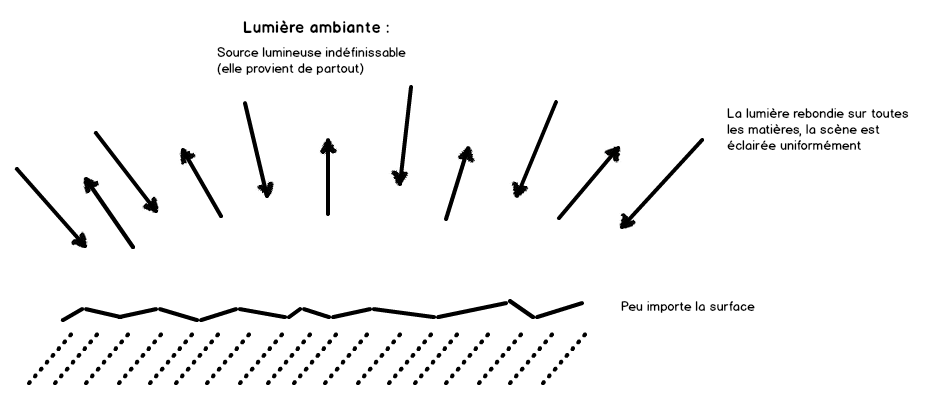
\includegraphics[width=17cm,height=7cm]{pipeline/images/lumiere_ambiante.png}
\end{center}

\section{Lumière diffuse}
\begin{center}
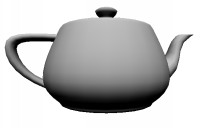
\includegraphics[width=5cm,height=5cm]{pipeline/images/objet_diffuse.png}
\end{center}
Cette composante provient d'une source précise, telle qu'une lampe, ou le soleil.
\\\\
Une lumière est diffuse quand sa réflexion sur la surface qu'elle éclaire n'est pas parfaite.
\\\\
On voit donc apparaître un reflet brillant quand elle touche l'objet. Elle est réfléchie à partir de l'objet dans toutes les direction de la scène.
\\\\
\begin{center}
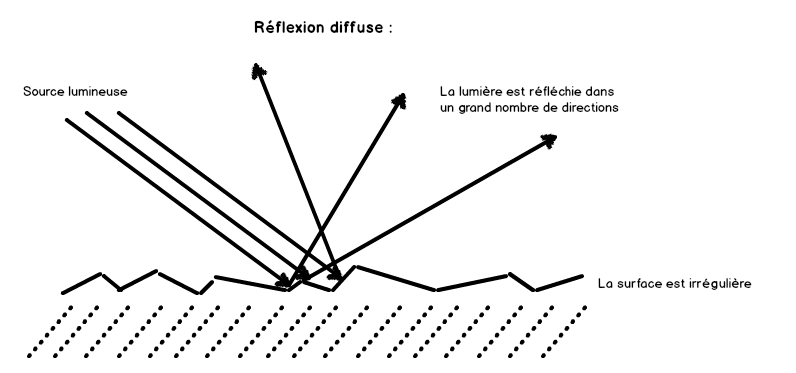
\includegraphics[width=17cm,height=7cm]{pipeline/images/reflexion_diffuse.png}
\end{center}

\section{Lumière spéculaire}
\begin{center}
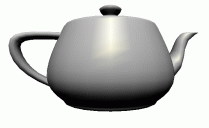
\includegraphics[width=5cm,height=5cm]{pipeline/images/objet_speculaire.png}
\end{center}
Cette composante qui arrive d'une direction et qui rebondit sur la surface en fonction des propriétés de l'objet et de son orientation par rapport à la source.
\\\\
\begin{center}
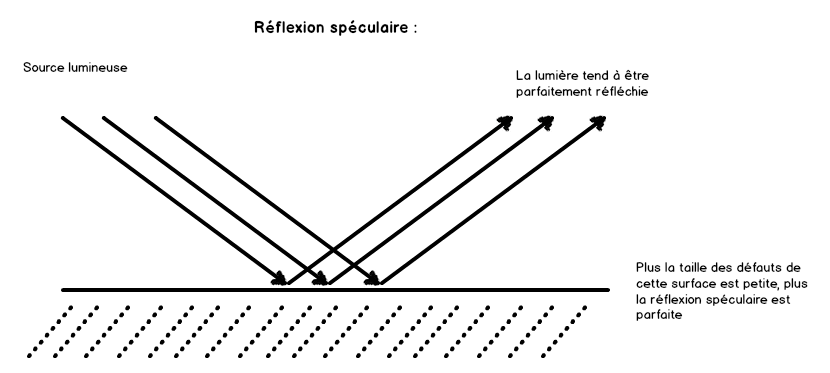
\includegraphics[width=17cm,height=7cm]{pipeline/images/reflexion_speculaire.png}
\end{center}

\section{Lumière émissive}
Cette composante est la lumière provenant d'un objet.
\\\\
Elle permet d'ajouter de l'intensité à un objet.
Elle n'affecte pas et n'est pas affecté par les autres composantes.
\\\\
\begin{center}
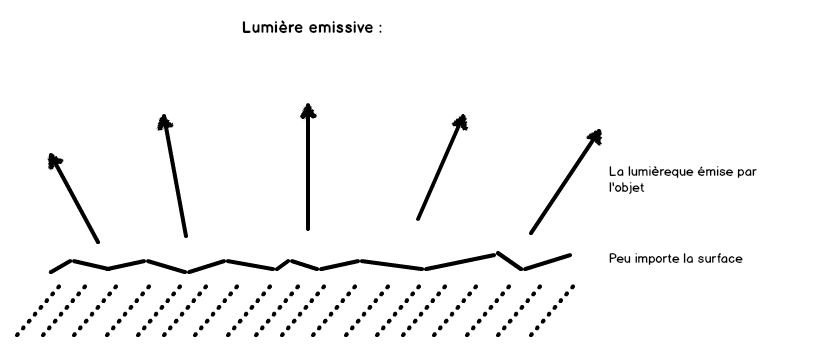
\includegraphics[width=17cm,height=7cm]{pipeline/images/lumiere_emissive.png}
\end{center}